%% Lee
%% In dissertation, change section* to chapter and subsection* to section

\chapter{State of the Art}
%\section{State of the Art}
\label{chap-two}

For the most part, large scale ANNs have been implemented using GPU's.
In some cases, these GPU's have demonstrated efficacy in the highly parallel processing required for some specific NNs such as Convolutional NNs.
There are also custom implementations that have targeted specific ANNs\cite{chen201614}\cite{farabet2011neuflow}, 
again such as convolutional neural networks (CNN). In most cases, these implementations focus on
solving specific "hot-spots" inherent in the processing of the network\cite{chen201614}.
%% Dissertation
\iffalse
%% convnets use shared parameters that 
%% a) help with translation invariance
%% b) reduce parameter space
%% CNNs are not always used in face recognition \cite{Taigman_2014_CVPR}
\fi
Almost all ASIC solutions employ arrays of processing elements (PE) each with local processing capability and local memory.
For most of these, the size of the network supported is limited by the size of the local memory and this large
local memory limits the number of available processing functions. % (MAC etc.).
In some cases \iftrue, as seen in \fref{fig:Example state-of-the-art die}\fi the area consumed for local memory can exceed of the order of 65\% of the 
processing element die \cite{kim2016neurocube}\cite{chen2014diannao}.
Those that employ external DRAM, such as NnSP{\cite{esmaeilzadeh2005nnsp} and NeuroCube\cite{kim2016neurocube} still 
load weights and inputs to local SRAM prior to processing.
In the case of NnSP{\cite{esmaeilzadeh2005nnsp}, the paper discusses caching data to bridge the speed gap between external memory and the PE 
but does not provide details on how to ensure data locality when reading a DRAM cacheline and how to minimize the impact of the DRAM protocol.
%% dissertion - mention overlapping kernels etc. ????
%%NnSP recognizes the need to stream from SDRAM but does not address the significant issues associated with
%%data structures in DRAM to facilitate streaming and minimize the access protocol limitations of DRAM.
NnSP does not provide any detail regarding network size and supported types.
Neuflow\cite{farabet2011neuflow} is limited to CNNs and the external memory is QDR SRAM 
and thus will be limited by the network size.
NeuroCube uses a 3D stack along with HMC 3D-DRAM and data is transferred from the DRAM to the PE's via a network-on-chip (NoC).
The combination of limited HMC interface bandwidth and the NoC limits the processing performance.
%%NeuroCube appears to transfer operands as packets so is not a "stream" processor.
Eyeriss\cite{chen201614} focuses on CNNs and specifically on the convolution "hot-spots". It does not support the pooling operations although these can
be supported by a local CPU but it does not support the memory intensive classifier stage. 
Eyeriss can not be effectively applied to locally-connected type ANNs such as Deepface \cite{Taigman_2014_CVPR}.

%% Dissertation
%\iffalse
\iftrue
Unlike the current state-of-the-art, this work focuses on processing data directly as that data is read out of the DRAM thus avoiding requiring excessive SRAM
in the PE's thus allowing optimum logic assignment to the processing functions.

To reiterate, state-of-the-art does not:
\vspace{-3mm}
\begin{itemize}
  \itemsep-1.5mm
  \item currently propose streaming data directly from 3D-DRAM through the processing functions to avoid the use of large local memory
  \item propose data structures to support continuous streaming from DRAM
  \item propose a 3D-stack supporting more than one processing layer
%%  \item provide specific special streaming functions to support a family of ANNs
\end{itemize}
%%%

%% Dissertation
\vspace{-1mm}
\begin{figure}
\centering
\begin{subfigure}{.45\textwidth}
  \centering
  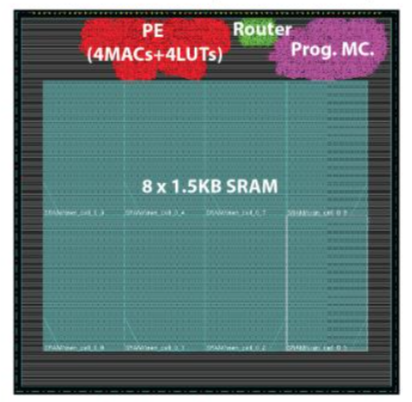
\includegraphics[width=0.8\textwidth]{Chapter-2/figs/kim2016neurocube_fig4}
  \captionsetup{justification=centering, skip=6pt}
  \caption{NeuroCube}
  \label{fig:NeuroCubeDie}
\end{subfigure}%
\begin{subfigure}{.45\textwidth}
  \centering
  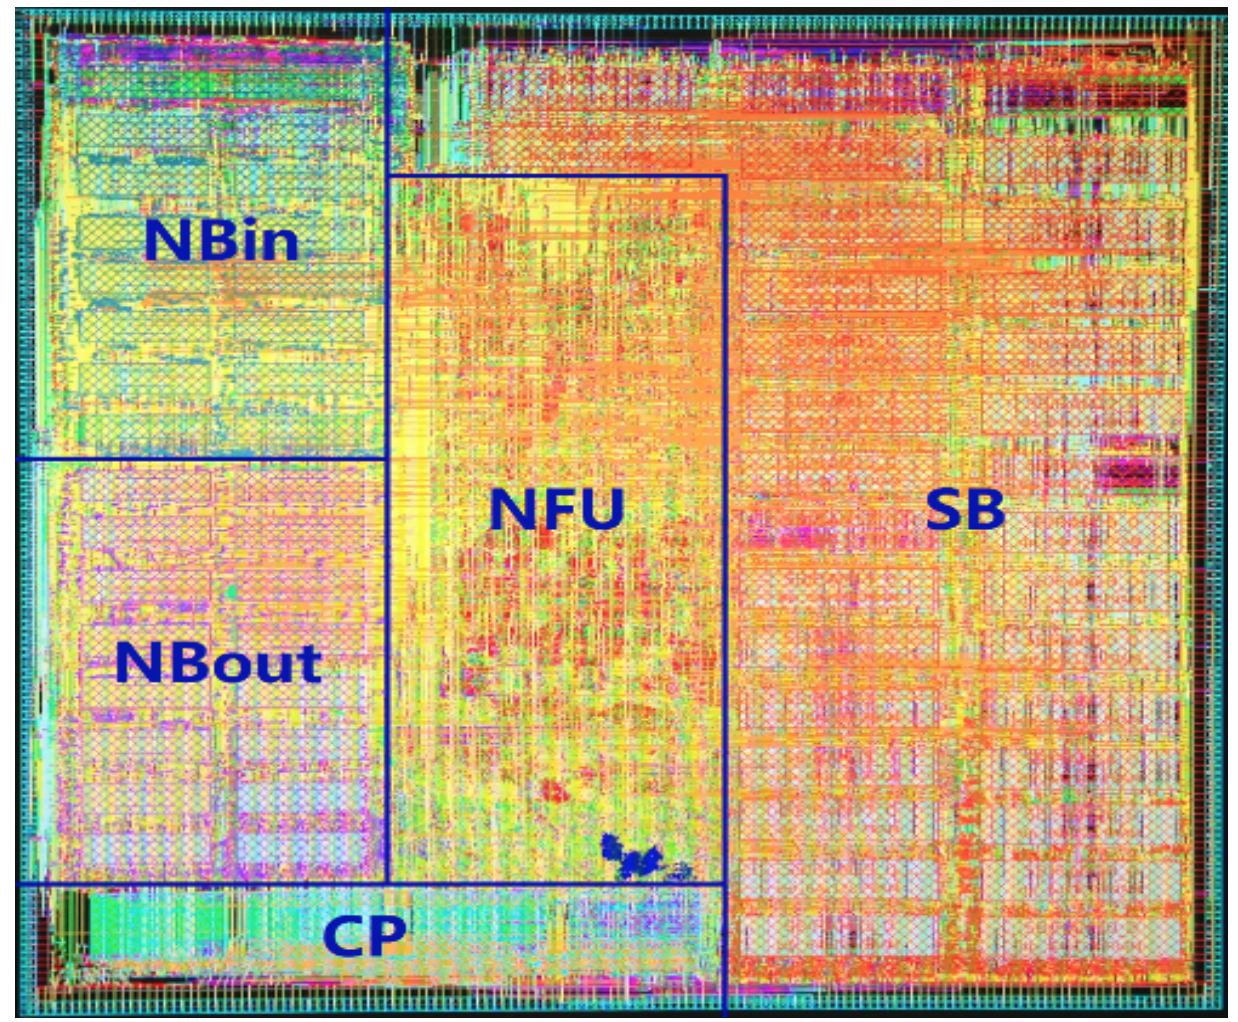
\includegraphics[width=0.8\textwidth]{Chapter-2/figs/chen2014diannao_fig15}
  \captionsetup{justification=centering, skip=10pt}
  \caption{Diannao (SB and NBx are SRAM)}
  \label{fig:DiannaoDie}
\end{subfigure}
\captionsetup{justification=centering, skip=3pt}
\caption{Example state-of-the-art die}
\label{fig:Example state-of-the-art die}
\end{figure}
\vspace{-5mm}
\fi


%% Uncomment for dissertation
\iftrue

\vspace{5mm}
NeuroCube\cite{kim2016neurocube} is the only solution to explicitly discuss 3D-memory but will again be limited by its focus on utilizing local SRAM where our focus is on
providing silicon for processing and not local storage.
Neuflow\cite{farabet2011neuflow} has processing elements that are limited to CNNs.
The Tensor processing Unit (TPU) \cite{jouppi2017datacenter} employs an array of eight bit processing elements but specifically states it is bandwidth limited with fully connected (MLP) networks
NnSP{\cite{esmaeilzadeh2005nnsp} transfers weights and inputs to local PE memory prior to processing.
nn-X\cite{gokhale2014240} limits the number format to integer, and although there is some acceptance that similar
results can be obtained compared to floating point, this will likely limit the applcation space. 
nn-X is also limited to performing the convolution operation and SRAM size will limit its capability when performing the classifier stage.

Below is a summary of current technology.

\section[NnSP]{NnSP{\cite{esmaeilzadeh2005nnsp}}}

Uses external DRAM with a cache.
 Does not address the main issue of DRAM access limitations and providing data structures.
 It simply says "use a cache" but doesnt justify locality issues.

Transfers weights and inputs to local PE prior to processing
Similar "Streaming" terminlogy but streams from local memory.
Neuron outputs are kept locally and transferred to other neurons thru NoC

Implemented in FPGA

No detail on processing element but likely limited to "standard" feedforward NN's


%% Note: add \section[<section>]{<section> \cite{}} instead of \section{<section> \cite...}
%% to avoid case mismatch issues when running bibtex
\section[NeuroCube]{NeuroCube{\cite{kim2016neurocube}}}
NeuroCube\cite{kim2016neurocube} transfers data to PE prior to processing which can limit classifier size although most
convolution kernels can be supported.
The SRAM on the PE is significant (see \fref{fig:NeuroCubeDie}).
NeuroCube uses HMC 3D-DRAM which has limited bandwidth and this will limit network processing performance.
The NeuroCube implements a processing layer but does not address adding additional layers. 

3D uses HMC
 - limited by HMC bandwidth
 - is serdes a good choice for die-to-die communication (typically used for die to chip/board?)
 - doesnt really discuss adding additional layers

Transfers data to PE prior to processing


\section[IMAPCAR]{IMAPCAR \cite{kyo2011imapcar}}
IMAPCAR uses external SRAM so will be limited by network size.
The architecture of IMAPCAR is optimized for processing video.

In general will not scale to ANNs of interest.


\section{NeuFlow \cite{farabet2011neuflow}}
Neuflow\cite{farabet2011neuflow} has processing elements that are "highly optimized" to CNNs.
Neuflow is designed around external QDR memory and does not address the issues associated with supporting large networks.


\section[nn-X]{nn-X \cite{gokhale2014240}}
nn-X\cite{gokhale2014240} limits the number format to integer, and although there is some acceptance that similar
results can be obtained, this will likely limit the applcation space. nn-X is also limited to performing the convolution operation
and SRAM size will limit its capability when performing the classifier stage.
nn-X was implemented in an fpga and does not address SRAM size when scaling to larger networks.


\section[Diannao]{Diannao \cite{chen2014diannao}}
Diannao\cite{chen2014diannao} acknowledges the need for large amounts of storage which will exceed the capability of local memory.
The kernel sizes are limited by SRAM size although it does state kernels can be "broken up".
The SRAM use on the PE is significant (see \fref{fig:DiannaoDie}).


\section[Eyeriss]{Eyeriss \cite{chen201614}}
Eyeris\cite{chen201614} focuses on CNNs and specifically the convolution stage.
Eyeriss ignores the pooling and classifier stages which although not as compute intensive they are memory intensive.
Therefore Eyeriss limits network size and does not implement the network.

\section[TPU]{TPU \cite{jouppi2017datacenter}}
The TPU utilizes an array of 256 processing elements and demonstrates significant (~30X) performance improvements over GPUs and CPUs. It does employ DRAM which provides the required storage capacity
but employs SRAM as an intermediate store between the DRAM and the PEs.
This Google designed solution acknowledges that it is bandwidth limited when implementing the fully connected MLP type NNs.
It also states that their experience of implementing NNs in the Google server farms suggests that these fully connected NNs represent the bulk of their processing requirements.
The simpler CNNs only represent 5\% of the servers NN processing requirements.
It should also be stated that this paper also believes that GPU solutions cannot reach the performance targets even though the GPU community might state otherwise.

\fi



%%%%%%%%%%%%%%%%%%%%%%%%%%%%%%%%%%%%%%%%%%%%%%%%%%%%%%%%%%%%%%%%%%%%%%%%%%%%%%%%%%%%%%%%%%%%%%%%%%%%%%%%%%%%%%%%%%%%%%%
%%%%%%%%%%%%%%%%%%%%%%%%%%%%%%%%%%%%%%%%%%%%%%%%%%%%%%%%%%%%%%%%%%%%%%%%%%%%%%%%%%%%%%%%%%%%%%%%%%%%%%%%%%%%%%%%%%%%%%%
%%%%%%%%%%%%%%%%%%%%%%%%%%%%%%%%%%%%%%%%%%%%%%%%%%%%%%%%%%%%%%%%%%%%%%%%%%%%%%%%%%%%%%%%%%%%%%%%%%%%%%%%%%%%%%%%%%%%%%%
%%%%%%%%%%%%%%%%%%%%%%%%%%%%%%%%%%%%%%%%%%%%%%%%%%%%%%%%%%%%%%%%%%%%%%%%%%%%%%%%%%%%%%%%%%%%%%%%%%%%%%%%%%%%%%%%%%%%%%%
%%%%%%%%%%%%%%%%%%%%%%%%%%%%%%%%%%%%%%%%%%%%%%%%%%%%%%%%%%%%%%%%%%%%%%%%%%%%%%%%%%%%%%%%%%%%%%%%%%%%%%%%%%%%%%%%%%%%%%%
